\section{Staging}\label{sec:staging}

\begin{frame}[c]
    \slidehead
    \centering
    \begin{tikzpicture}
        \node[node_inactive] (clean) {working tree clean};
        \node[node_inactive, fill=red!10!gray, below=2.5em of clean] (modified) {modified};
        \node[node_inactive, fill=green!10!gray, below=2.5em of modified] (staged) {staged};

        \node[tiny-commit, above right=-3em and 10em of staged] (a1){};
        \node[tiny-commit, right=5em of a1] (b1){};

        \node[tiny-commit, above=2em of a1] (a2){};
        \node[tiny-commit, above=2em of b1] (b2){};

        \node<6->[tiny-commit, fill=TUDa-8a, above=2em of a2] (a3){};
        \node<7->[tiny-commit, fill=TUDa-8a, above=2em of b2] (b3){};

        \draw<6->[parent] (a3) to (a2);
        \draw[parent] (a2) to (a1);
        \draw<7->[parent] (b3) to (b2);
        \draw[parent] (b2) to (b1);

        \draw<7>[parent] (a3) to node[above, pos=0.5] {\texttt{push}} (b3);
        \draw<8>[parent] (b3) to node[above, pos=0.5] {\texttt{pull}} (a3);

        \node[above=6em of a2, text width=3em, align=center] (localrepo) {Local Repo};
        \node[above=6em of b2, text width=3em, align=center] (remoterepo) {Remote Repo};

        \draw[parent-inactive] (clean.south) -- (modified.north) node[right, pos=0.5] {\texttt{modify}};
        \draw[parent-inactive] (modified.south) -- (staged.north) node[right, pos=0.5] {\texttt{git add}};
        \draw[parent-inactive] (staged) to[out=0, in=0, looseness=2] node[right, pos=.5] {\texttt{modify}} (modified);
        \draw[parent-inactive] (staged) to[out=180,in=180, looseness=1.5] node[left, pos=.5] {\texttt{git commit}} (clean);

        \node<2,5->[node] (clean-active) at (clean) {working tree clean};
        \node<3,5->[node, fill=red!50!gray] (modified-active) at (modified) {modified};
        \node<4,6->[node, fill=green!40!gray] (staged-active) at (staged) {staged};

        \draw<3,6->[parent] (clean.south) -- (modified.north) node[right, pos=0.5] {\texttt{modify}};
        \draw<4,6->[parent] (modified.south) -- (staged.north) node[right, pos=0.5] {\texttt{git add}};
        \draw<5->[parent] (staged) to[out=0, in=0, looseness=2] node[right, pos=.5] {\texttt{modify}} (modified);
        \draw<5->[parent] (staged) to[out=180,in=180, looseness=1.5] node[left, pos=.5] {\texttt{git commit}} (clean);
    \end{tikzpicture}
\end{frame}

\begin{frame}
    \slidehead
    \vspace{-1em}
    \centering
    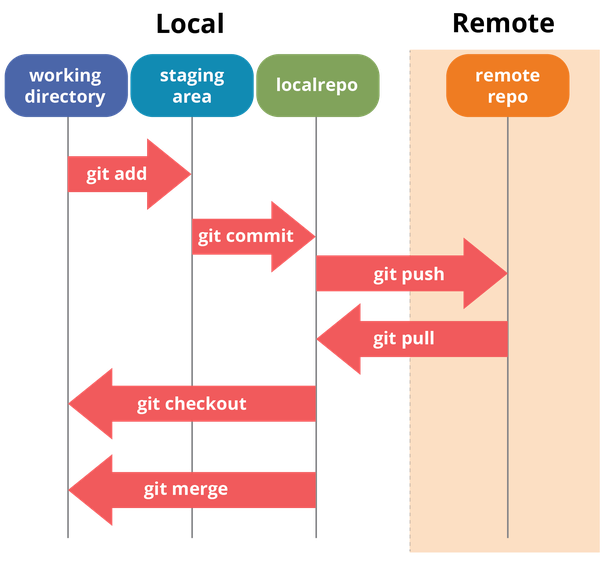
\includegraphics[scale=.3]{../pictures/structure-overview}
\end{frame}
